\section{Experiments}\label{sec:experiments}
In this section we examine the effectiveness of our invariant layer by testing
its performance on the well known datasets (listed in the order of increasing
difficulty):
\begin{itemize}
  \item MNIST: 10 classes, 6000 images per class, $28\x 28$ pixels per image.
  \item CIFAR-10: 10 classes, 5000 images per class, $32\x 32$ pixels per image.
  \item CIFAR-100: 100 classes, 500 images per class, $32\x 32$ pixels per image. 
  \item Tiny ImageNet\cite{li_tiny_nodate}: 200 classes, 500 images per class, 
    $64 \x 64$ pixels per image. 
\end{itemize}
Our experiment code is available at
\url{https://github.com/fbcotter/invariant_convolution}.

\subsection{Layer Introduction with MNIST}\label{sec:ch5:mnist}
To begin experiments on the proposed locally invariant layer, we look at how
well a simple system works on MNIST, and compare it to an equivalent system with
convolutions. To minimize the effects of learning from other layers, we build a
custom small network, as described in \autoref{tab:ch5:mnist_arch}.

The first two layers are learned convolutional/invariant layers, followed by a fully connected 
layer with fixed weights that we can use to project down to the number of output
classes. Finally, we add a small learned layer that linearly combines the 10
outputs from the random projection, to give 10 new outputs. This is to
facilitate reordering of the outputs to the correct class. This simple network is
meant to test the limits of our layer, rather than achieve state of the art
performance on MNIST.

Given that our layer is quite different to a standard convolutional layer, we
must do a full hyperparameter search over optimizer parameters such as the
learning rate, momentum, and weight decay, as well layer hyperparameters 
such as the variance of the random initialization for the mixing matrix $A$.

To simplify the weight variance search, we use Glorot Uniform Initialization
\cite{glorot_understanding_2010} and only vary the gain value $a$:
%
\begin{equation}
  A_{ij} \drawnfrom U\left[ -a\sqrt{\frac{6}{(C_l + C_{l+1})HW}},\ a\sqrt{\frac{6}{(C_l + C_{l+1})HW}}\
  \right] \label{eq:ch5:glorot}
\end{equation}
%
where $C_l,\ C_{l+1}$ are the number of input and output channels as before, and
the kernel size is $H = W = 1$ for an invariant layer and $H = W= 3$ for a
convolutional layer.

We do a grid search over these hyperparameters and use Hyperband
\cite{li_hyperband:_2016} to schedule early stopping of poorly performing runs.
Each run has a grace period of 5 epochs and can train for a maximum of 20
epochs. We do not do any learning rate decay.  We found the package Tune \cite{liaw2018tune}
was very helpful in organising parallel distributed training runs.  
% Finally, we use fANOVA \cite{hutter_efficient_2014} analysis
% to find the importance of these hyperparameters to our layer, comparing to a
% standard layer. 
The hyperparameter options are described in
\autoref{tab:ch5:hyper_options}, note that we test $4^4=256$ different options.

Once we find the optimal hyperparameters for each network, we then run the two
architectures 10 times with different random seeds and report the mean and variance of
the accuracy. The results of these runs are listed in
\autoref{tab:ch5:mnist_initial_results}.

\begin{table}[t]
  \renewcommand{\arraystretch}{1.4}
  \centering
  \mycaption{Architectures for MNIST hyperparameter experiments}{The activation
  size rows are offset from the layer description rows to convey the input and
  output shapes. The project layers in both architectures are unlearned, so all
  of the learning has to be done by the first two layers and the reshuffle
  layer.}
  \label{tab:ch5:mnist_arch}
  \subfloat[Invariant Architecture]{%
    \label{tab:ch5:mnist_arch_inv}
    \begin{tabular}{c c}
      \toprule
      Activation Size & Layer Name + Info \\
      \midrule
      \begin{tabular}{@{}c@{}} % This supresses the space on the left and right
        $1\x 28 \x 28$ \\ $7\x 14\x 14$ \\ $49\x 7\x 7$ \\ $2401\x 1$ \\ $10\x 1$
        \\ $10\x 1$ 
      \end{tabular} &
      \begin{tabular}{@{}c@{}}
        inv1, $A \in \reals[7\x 7]$ \\ inv2, $A \in \reals[49\x 49]$ \\ unravel \\
        project, $w \in \reals[2401\x 10]$ \\ reshuffle, $w\in \reals[10\x 10]$
      \end{tabular}\\
      \bottomrule
    \end{tabular}
  }\quad
  \subfloat[Reference Arch with $3\x 3$ convolutions]{%
    \label{tab:ch5:mnist_arch_conv}
    \begin{tabular}{c c}
      \toprule
      Activation Size & Layer Name + Info \\
      \midrule
      \begin{tabular}{@{}c@{}} % This supresses the space on the left and right
        $1\x 28 \x 28$ \\ $7\x 28\x 28$ \\ $7\x 14\x 14$ \\ $49\x 14\x 14$ \\ $49\x 7\x 7$ 
        \\ $2401\x 1$ \\ $10\x 1$ \\ $10\x 1$ 
      \end{tabular} &
      \begin{tabular}{@{}c@{}}
        conv1, $w \in \reals[7\x 1\x 3 \x 3]$ \\ maxpool1, $2\x 2$ \\ 
        conv2 $w \in \reals[49\x 7 \x 3\x 3]$ \\ maxpool2, $2\x 2$ \\ unravel \\
        project, $w \in \reals[2401\x 10]$ \\ reshuffle, $w\in \reals[10\x 10]$
      \end{tabular} \\
      \bottomrule
    \end{tabular}
  }
\end{table}

\begin{table}[hbt]
  \centering
  \mycaption{Hyperparameter settings for the MNIST experiments}{The weight gain is
  the term $a$ from \autoref{eq:ch5:glorot}. Note that $\log_{10} 3.16 = 0.5$.}
  \label{tab:ch5:hyper_options}
  \begin{tabular}{c c}
    \toprule
    Hyperparameter & Values \\
    \midrule
    Learning Rate (lr) & $\left\{ 0.0316,\ 0.1,\ 0.316,\ 1 \right\}$ \\
    Momentum (mom) & $\left\{ 0,\ 0.25,\ 0.5,\ 0.9 \right\}$ \\
    Weight Decay (wd) & $\left\{ 10^{-5},\ 3.16\x 10^{-5},\ 10^{-4},\ 3.16\x 10^{-4} \right\} $\\
    Weight Gain (a) & $\left\{0.5,\ 1.0,\ 1.5,\ 2.0 \right\}$
    \\\bottomrule
  \end{tabular}
\end{table}

\begin{table}[hbt]
  \centering
  \mycaption{Architecture performance comparison}{Numbers reported are the mean
  and standard deviation of accuracy over 10 runs with the optimal
  hyperparameters, $\theta$. Note that for
  both architectures we found that $\F{lr}$ was the most important
  hyperparameter to choose correctly, and had the largest impact on the
  performance.
  % We also use
  % fANOVA\cite{hutter_efficient_2014} analysis to weight the importance of these 
  % hyperparameters. High values imply the accuracy is more sensitive to this
  % hyperparameter. 
  }
  \label{tab:ch5:mnist_initial_results}
  \begin{tabular}{@{}l c c c@{}}
    \toprule
     & &\multicolumn{2}{c}{accuracy} \\\cline{3-4}
    Architecture & $\theta = \{\F{lr}, \F{mom}, \F{wd}, \F{a}\}$ & mean & std  \\\midrule
    Convolutional & $\{0.1,\ 0.5,\ 10^{-5},\ 1.5 \}$ & 97.3 & 0.29 \\
    Invariant & $\{0.032,\ 0.9,\ 3.2\x 10^{-5},\ 1.0 \}$ & 96.6 & 0.26 \\
    \bottomrule
  \end{tabular}
\end{table}

\subsubsection{Proposed Expansions}\label{sec:ch5:mnist_initial}
The results from the previous section seem to indicate that
our proposed invariant layer is a slightly worse substitute for a convolutional
layer. However we believe that this is due to the centred nature of the wavelet bases that were
used to generate the $z$ and later the $y$ coefficients. A similar effect was seen
in the previous chapter in \autoref{fig:ch4:shapes} where the space of shapes
attainable by mixing wavelet coefficients in a $3\x 3$ area was much richer than
those attainable by only mixing in a $1\x 1$ area. 

% \begin{figure}[t]
  % \centering
  % \subfloat[Invariant Layers]{%
  % 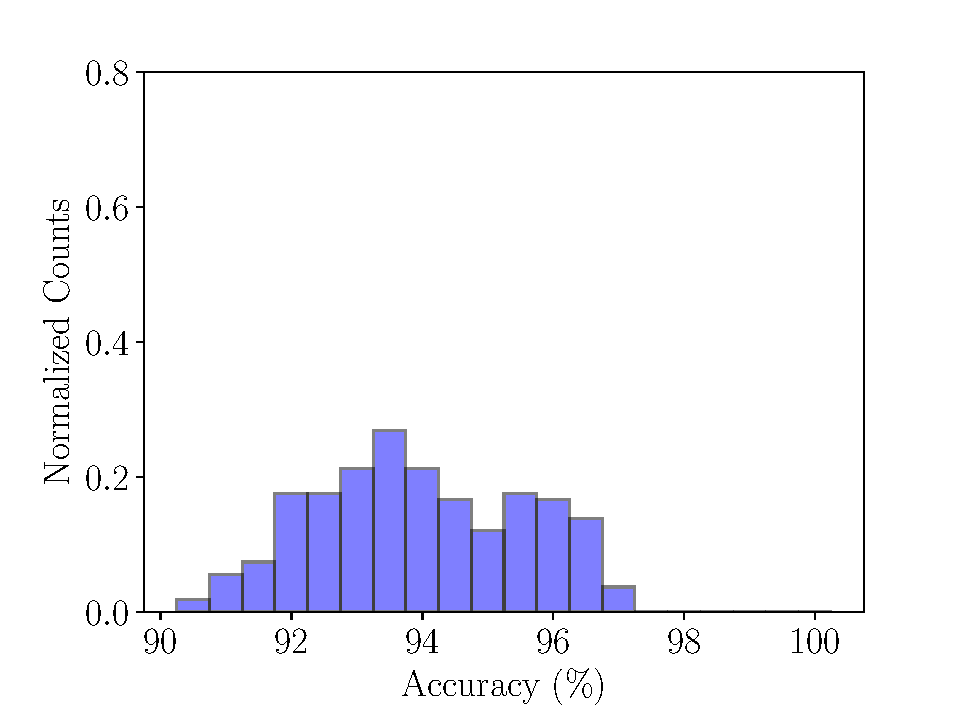
\includegraphics[width=0.5\linewidth]{\imgpath/mnist_inv1x1_grid.pdf}
  % \label{fig:ch5:mnist_comparison_inv}
  % }
  % \subfloat[Convolutional Layers]{%
  % 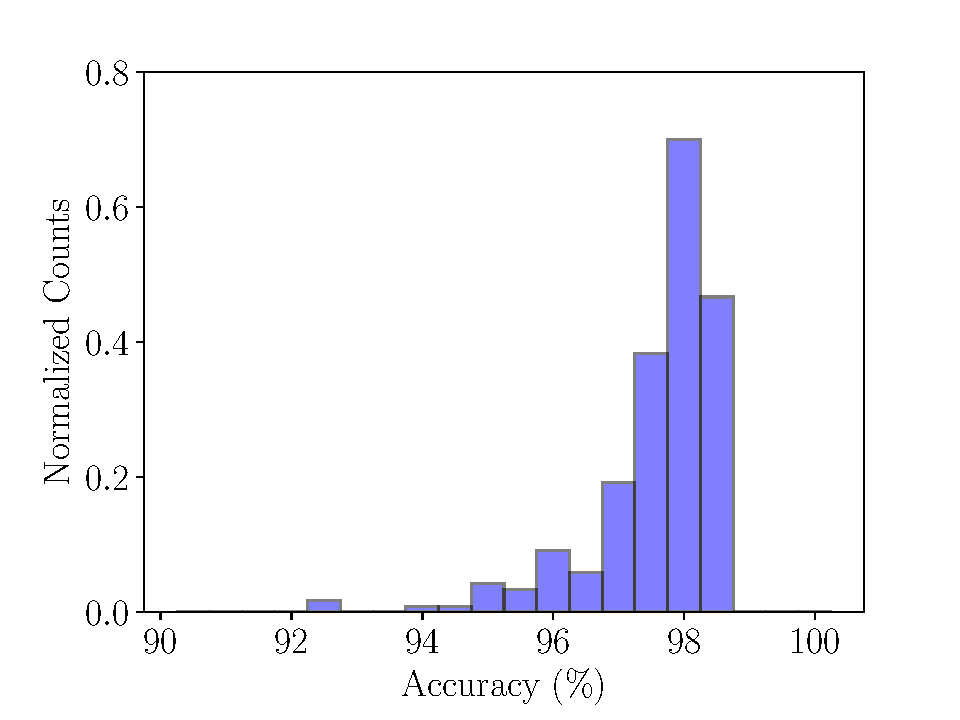
\includegraphics[width=0.5\linewidth]{\imgpath/mnist_conv3x3_2.pdf}
  % \label{fig:ch5:mnist_comparison_conv}
  % }
  % \mycaptionnodot{Histogram of classification accuracies}{for the two architectures from
  % \autoref{tab:ch5:mnist_arch} over 256 runs with varying hyperparameters. 
  % The proposed invariant layer is more sensitive
  % to hyperparameters and overall worse performing than the architecture with
  % standard $3\x 3$ convolutions.}
  % \label{fig:ch5:mnist_comparison}
% \end{figure}

To test this hypothesis, we change \autoref{eq:ch5:mixing} to be:
\begin{equation}
  y^{(l+1)}(f, \xy)  =  \sum_{q \in Q} z^{(l+1)}(q, \xy) \conv \left(\tilde{a}_f(q) \alpha_f(q, \xy) \right)
\end{equation}

Where $\alpha_f(q, \xy)$ is an introduced kernel designed to allow mixing of
wavelets from neighbouring spatial locations. We test a range of possible
$\alpha$'s each with varying complexity/overhead:

\begin{enumerate}[(a)]
  \item We randomly shift each of the $7C$ subbands horizontally
    by $\{-1, 0, 1\}$ pixels, and vertically by $\{-1, 0, 1\}$ pixels. This is
    determined at the beginning of a training session and is consistent between
    batches. This theoretically is free to do, but practically it involves
    convolving with a $3 \x 3$ kernel with a single $1$ and eight $0$'s.
  \item Instead of shifting impulses as in the previous option, we can shift a
    gaussian kernel by one pixel left/right and up/down, making a smoother filter. 
  \item Instead of imposing a lowpass/impulse structure, we can set $\alpha$ to
    be a random $3\x 3$ kernel. This is chosen once at the beginning of training and then
    is kept fixed between batches.
  \item We can set the $3\x 3$ kernel to be fully learned. This
    still makes for a novel layer, but now the parameter cost is 9 times higher
    than the $1\x 1$ conv layer, and 7 times higher than a vanilla $3\x 3$
    convolution.
  \item We can take the top three $3\x 3$ DCT coefficients of the $7C$
    subbands, allowing us to do something like the previous option 
    but with only a threefold parameter increase. The top three coefficients are
    the constant, the horizontal and the vertical filters.
\end{enumerate}

Again, we search over the hyperparameter space to find the optimal
hyperparameters and then run 10 runs at the best set of hyperparameters, and
report the results in \autoref{tab:ch5:mnist_new_results}. As we expected,
adding in random shifts significantly helps the invariant layer. Two systems of
note are the shifted impulse (a) system and the learned $3\x 3$ kernel (d)
system. The first improves the mean accuracy by $1.3\%$ without any extra
learning. The second improves the performance by $2.4\%$ but with a large
parameter cost. To explore an equivalent system, we also list in
\autoref{tab:ch5:mnist_new_results} a modification to the convolutional
architecture that uses $5\x 5$ convolutions and $C_1 = 10,\ C_2 = 100$ channels,
resulting in a system with comparable parameter cost to (d).

\begin{table}[hbt]
  \renewcommand{\arraystretch}{1.4}
  \centering
  \mycaption{Modified architecture performance comparison}{Numbers reported are the mean
  and standard deviation of accuracy over 10 runs with the optimal
  hyperparameters, $\theta$. We also list parameter cost and number
  of multiplies for each layer option, relative to the standard $3\x 3$
  convolutional layer to highlight the benefits/drawbacks of each option.}
  \label{tab:ch5:mnist_new_results}
  \begin{tabular}{@{}l c c c c c@{}}
    \toprule
    & & \multicolumn{2}{c}{cost} & \multicolumn{2}{c}{accuracy} \\\cline{3-4}\cline{5-6}
    Architecture & $\theta = \{\F{lr}, \F{mom}, \F{wd}, \F{a}\}$ & param & mults & mean & std  \\\midrule
    Convolutional & $\{0.1,\ 0.5,\ 10^{-5},\ 1.5 \}$ & 1 & 1 & 97.3 & 0.29 \\
    Invariant & $\{0.032,\ 0.9,\ 3.2\x 10^{-5},\ 1.0 \}$ & $\frac{7}{9}$ & $\frac{7}{36}$ & 96.6 & 0.26 \\\midrule
    Shifted impulses (a) & $\{0.32,\ 0.5,\ 10^{-4},\ 1.0 \}$ & $\frac{7}{9}$ & $\frac{7}{36}$ & 97.9 & 0.25 \\
    Shifted gaussians (b) & $\{1.0,\ 0.0,\ 10^{-5},\ 1.0 \}$ & $\frac{7}{9}$ & $\frac{7}{4}$ & 97.7 & 0.56\\
    Random $3\x3$ kernel (c) & $\{1.0,\ 0.9,\  10^{-5},\ 1.0 \}$ & $\frac{7}{9}$ & $\frac{7}{4}$ & 95.8 & 1.01\\
    Learned $3\x3$ kernel (d) & $\{0.1,\ 0.5,\  10^{-4},\ 1.0 \}$ & \textbf{7} & $\frac{7}{4}$ & \textbf{99.0} & 0.12 \\
    Learned 3 DCT coeffs (e) & $\{1.0,\ 0.0,\ 10^{-5},\ 1.0 \}$ & $\frac{7}{3}$ & $\frac{7}{4}$ & 98.1 & 0.37\\\midrule
    Wide Convolutional & $\{0.1,\ 0.5,\ 10^{-5},\ 1.5 \}$ & 7 & 7 &  &  \\
    \bottomrule
  \end{tabular}
\end{table}

% \subsubsection{Modified MNIST Results}
% The results of the new experiments are shown in
% \autoref{fig:ch5:mnist_comparison}. All options improve on the original
% performance seen in \autoref{fig:ch5:mnist_comparison_inv} proving that it is
% important to spatially separate the wavelets, something the original Scatternet
% design cannot do. Of particular interest are options
% \subref{fig:ch5:mnist_comparison_smooth},
% \subref{fig:ch5:mnist_comparison_3x3} and
% \subref{fig:ch5:mnist_comparison_dct}. \protect\subref{fig:ch5:mnist_comparison_smooth} 
% is the best performing option without increasing the parameter cost and is very
% near the reference architecture.
% \textbf{Finish me.}

% \begin{figure}[hbtp]
  % \centering
  % \subfloat[Randomly shifted impulse]{%
  % 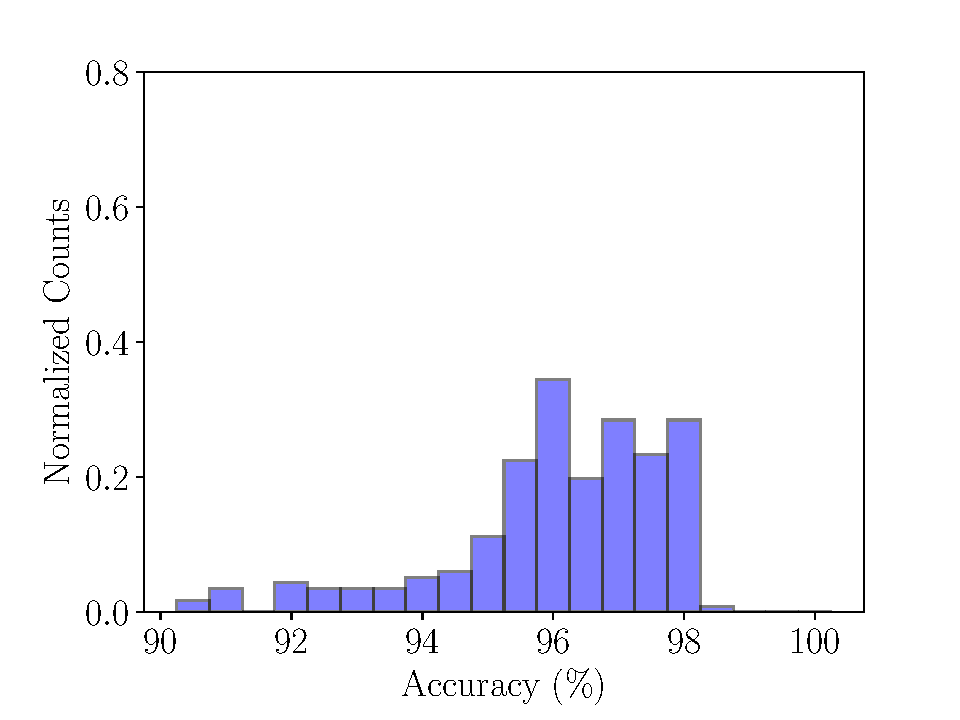
\includegraphics[width=0.45\linewidth]{\imgpath/mnist_inv1x1_random_impulse2.pdf}
  % \label{fig:ch5:mnist_comparison_impulse}
  % }
  % \subfloat[Randomly shifted $3\x 3$ gaussian]{%
  % 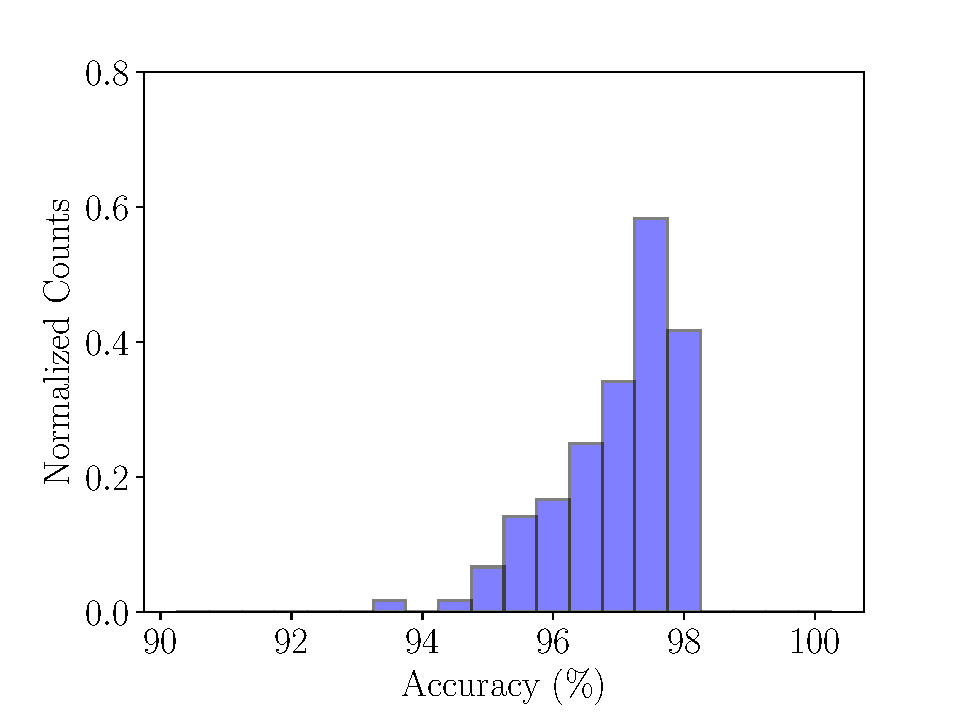
\includegraphics[width=0.45\linewidth]{\imgpath/mnist_inv1x1_random_smooth.pdf}
  % \label{fig:ch5:mnist_comparison_smooth}
  % }\\\vspace{-10pt}
  % \subfloat[Fixed random $3\x 3$ filter]{%
  % 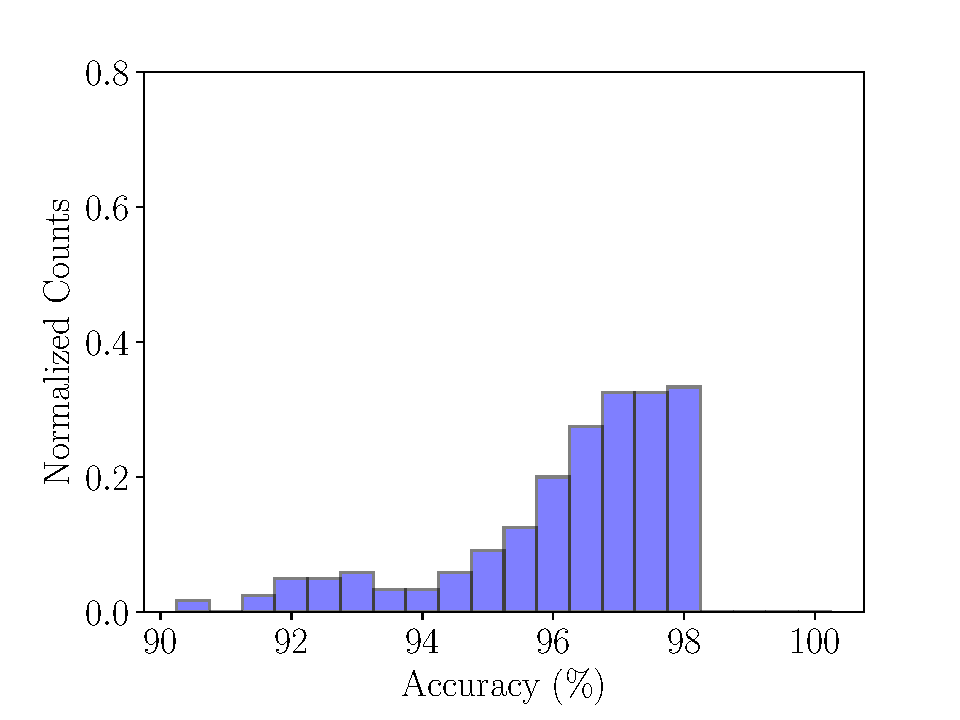
\includegraphics[width=0.45\linewidth]{\imgpath/mnist_inv1x1_random2.pdf}
  % \label{fig:ch5:mnist_comparison_random}
  % }
  % \subfloat[Fully learned $3\x 3$ $A$ matrix]{%
  % 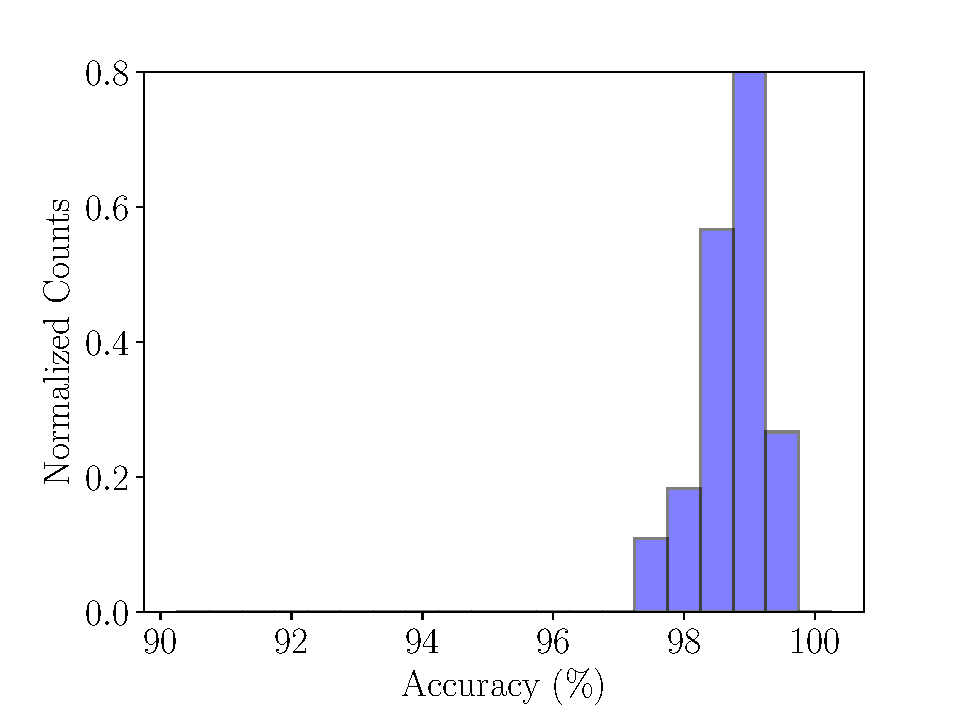
\includegraphics[width=0.45\linewidth]{\imgpath/mnist_inv3x3.pdf}
  % \label{fig:ch5:mnist_comparison_3x3}
  % }\\\vspace{-10pt}
  % \subfloat[Top three DCT coefficients]{%
  % 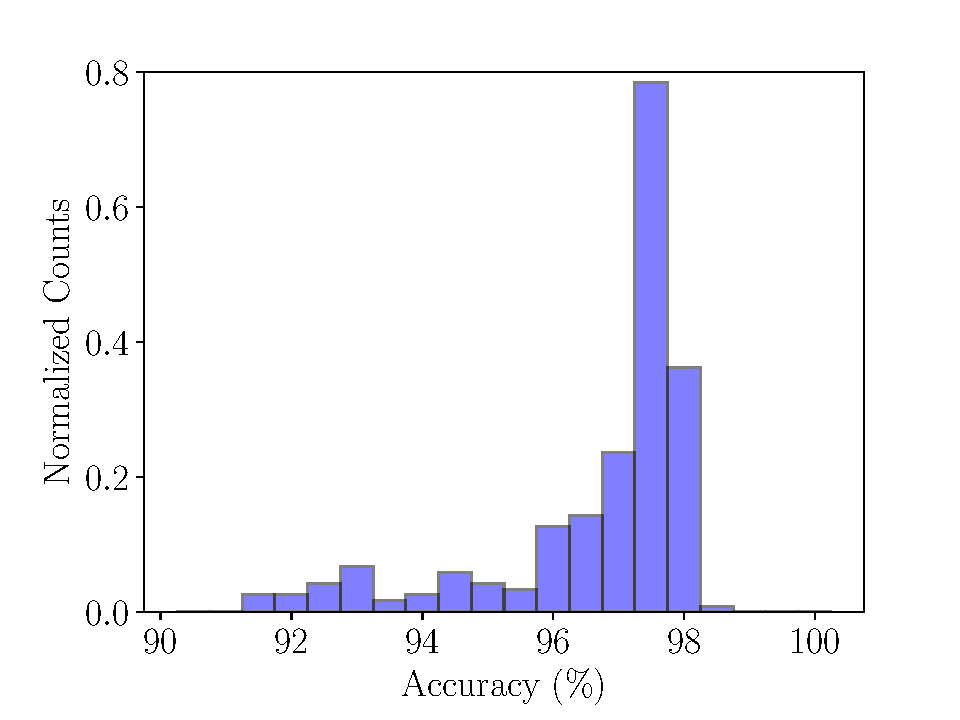
\includegraphics[width=0.45\linewidth]{\imgpath/mnist_inv1x1_dct.pdf}
  % \label{fig:ch5:mnist_comparison_dct}
  % }\\
  % \mycaptionnodot{Histogram of new classification accuracies}{for the five 
  % modified architectures presented in \autoref{sec:ch5:mnist_initial}. 
  % The subcaption describes the $\alpha$ kernel introduced to provide spatial separation
  % of wavelet coefficients.}
  % \label{fig:ch5:mnist_comparison}
% \end{figure}

% \subsubsection{Optimal Hyperparameters}


\subsection{Layer Comparison with CIFAR and Tiny ImageNet}\label{sec:conv_exp}
Now we look at expanding our layer to harder datasets, focusing more on the
final classification accuracy. We do this again by comparing to a reference
architecture based on VGG.
It has six convolutional layers for CIFAR and eight layers for Tiny ImageNet as shown in
\autoref{tab:arch}. The initial number of channels $C$ we use is 64. Despite
this simple design, this reference architecture achieves competitive performance
for the three datasets.

This network is optimized with stochastic gradient descent with momentum. The
initial learning rate is $0.5$, momentum is $0.85$, batch size $N=128$ and
weight decay is $10^{-4}$. For CIFAR-10/CIFAR-100 we scale the learning rate by
a factor of 0.2 after 60, 80 and 100 epochs, training for 120 epochs in total.
For Tiny ImageNet, the rate change is at 18, 30 and 40 epochs (training for 45 in total).

\begin{table}[ht]
  \centering
  \caption{Base Architecture used for Convolution Layer comparison tests.
  \textsuperscript{\textdagger}indicates only used in Tiny ImageNet
  experiments.}
  \label{tab:arch}
  \begin{tabular}{c|c}
    \textbf{Name} & \textbf{Output Size}  \\\hline
    convA & $C\x H\x W$ \\
    convB & $C\x H\x W$ \\
    convC & $2C\x H/2\x W/2$\\
    convD & $2C\x H/2\x W/2$\\
    convE & $4C\x H/4\x W/4$\\
    convF & $4C\x H/4\x W/4$\\
    convG\textsuperscript{\textdagger} & $8C\x H/8\x W/8$\\
    convH\textsuperscript{\textdagger} & $8C\x H/8\x W/8$\\
    fc & num classes \\
    % conv1\_1 & $C\x H\x W$ & conv+bn+ReLU\\
    % conv1\_2 & $C\x H\x W$ & conv+bn+ReLU+maxpool \\
    % conv2\_1 & $2C\x H/2\x W/2$& conv+bn+ReLU \\
    % conv2\_2 & $2C\x H/2\x W/2$& conv+bn+ReLU+maxpool \\
    % conv3\_1 & $4C\x H/4\x W/4$& conv+bn+ReLU \\
    % conv3\_2 & $4C\x H/4\x W/4$& conv+bn+ReLU+maxpool\textsuperscript{\textdagger} \\
    % conv4\_1\textsuperscript{\textdagger} & $8C\x H/8\x W/8$& conv+bn+ReLU \\
    % conv4\_2\textsuperscript{\textdagger} & $8C\x H/8\x W/8$& conv+bn+ReLU \\
    % fc1 & num classes & average pool + fc \\
    % conv1\_1 & conv $C\x 3\x 3\x 3$, bn+ReLU\\
    % conv1\_2 & conv $C\x C\x 3\x 3$, bn+ReLU, maxpool $2\x 2$ \\
    % conv2\_1 & conv $2C\x C\x 3\x 3$, bn+ReLU \\
    % conv2\_2 & conv $2C\x 2C\x 3\x 3$, bn+ReLU, maxpool $2\x 2$ \\
    % conv3\_1 & conv $4C\x 2C\x 3\x 3$, bn+ReLU \\
    % conv3\_2 & conv $4C\x 4C\x 3\x 3$, bn+ReLU maxpool\textsuperscript{\textdagger} $2\x 2$\\
    % conv4\_1\textsuperscript{\textdagger} & conv $8C\x 4C\x 3\x 3$, bn+ReLU \\
    % conv4\_2\textsuperscript{\textdagger} & conv $8C\x 8C\x 3\x 3$, bn+ReLU \\
    % fc1 & average pool $8\x 8$, fc $4C\x \F{num classes}$
  \end{tabular}
\end{table}



We perform an ablation study where we progressively swap out convolutional
layers for invariant layers keeping the input and output activation sizes the
same. As there are 6 layers (or 8 for Tiny ImageNet), there are too many
permutations to list the results for swapping out all layers for our locally
invariant layer, so we restrict our results to swapping 1 or 2 layers. 
\autoref{tab:conv_results} reports the top-1 classification accuracies for
CIFAR-10, CIFAR-100 and Tiny ImageNet. In addition to testing on the full
datasets we report results for a reduced training set size. In the table, `invX'
means that the `convX' layer from \autoref{tab:arch} is replaced with an 
invariant layer.

Interestingly, we see improvements when one or two invariant layers are used near the
start of a system, but not for the first layer. 
\begin{table}
  \renewcommand{\arraystretch}{1.2}
  \centering
  \caption{Results for testing VGG like architecture with convolutional and
  invariant layers on several datasets. An architecture with `invX' means the
  equivalent convolutional layer `convX' from \autoref{tab:arch} was swapped for
  our proposed layer.}
  % \begin{tabular}{@{}lllcllcll@{}}
  \begin{tabular}{@{}lcclcclcc@{}}
    \toprule
    & \multicolumn{2}{c}{CIFAR-10} & \phantom{abc} & \multicolumn{2}{c}{CIFAR-100} & \phantom{abc} & \multicolumn{2}{c}{Tiny ImgNet} \\ \cline{2-9}
    \phantom{abc} & 10k   &  50k  &&  10k  &  50k && 20k & 100k \\ \midrule
    reference arch & 84.4  & 91.9  && 53.2  & 70.3 && 37.4 & 59.1 \\ \hline
    invA & 82.8 & 91.3 && 48.4 & 69.5 && 33.2 & 57.7 \\
    invB & 84.8 & 91.8  && 54.8  & 70.7 && 36.9& 59.5 \\
    invC & 85.3 & 92.3 && 54.2 & 71.2 && 37.1& 59.8\\
    invD& 83.8 & 91.2 && 51.2 & 70.1 && 37.6 & 59.3 \\
    invE& 83.3 & 91.6 && 50.3 & 70.0 && 37.8 & 59.4\\
    invF& 82.1 & 90.5 && 47.6& 68.9 && 34.0 & 57.8\\ \hline
    invA, invB& 83.1  & 90.5 && 49.8 & 68.4 && 35.0 & 57.9\\
    invB, invC& 83.8  & 91.2 && 50.6 & 69.1 && 34.6 & 57.5\\
    invC, invD& 85.1 & 92.1 && 54.3 & 70.1 && \textbf{37.9} & 59.0\\
    invD, invE& 80.2 & 89.1 && 49.0 & 67.3 && 33.9 & 57.5\\
    invA, invC& 82.8 & 90.7 && 49.5 & 69.6 && 34.0 & 56.9\\
    invB, invD& \textbf{85.4} & \textbf{92.7} && \textbf{54.6} & \textbf{71.3} && \textbf{37.9} & 59.8\\
    invC, invE& 84.8 & 91.8 && 53.5 & 70.9 && 37.6 & \textbf{60.2}\\ \bottomrule
  \end{tabular}\label{tab:conv_results}
\end{table}



\subsection{Network Comparison}\label{sec:scat_exp}
In the previous section, we examined how the locally invariant layer performs when
directly swapped in for a convolutional layer in an architecture designed
for convolutional layers. In this section, we look at how
it performs in a Hybrid ScatterNet-like \cite{oyallon_hybrid_2017,oyallon_scaling_2017},
network.

To build the second order ScatterNet, we stack two invariant layers on top of each
other. For 3 input channels, the output of these layers has $3(1 +
6 + 6 +36) = 147$ channels at $1/16$ the spatial input size. We then use 4
convolutional layers, similar to convC to convF in \autoref{tab:arch} with
$C=96$. In addition, we use dropout after these later convolutional layers with drop probability $p=0.3$.

We compare a ScatterNet with no learning in between scattering orders
(ScatNet A) to one with our proposal for a learned mixing matrix $A$ (ScatNet B). Finally,
we also test the hypothesis seen from \autoref{sec:conv_exp} about putting conv
layers before an inv layer, and test a version with a small convolutional layer
before ScatNets A and B, taking the input from 3 to 16 channels, and call these ScatNet
architectures ScatNet C and D respectively.

See \autoref{tab:hybrid_scat} for results from these experiments. It is clear from
the improvements that the mixing layer helps the Scattering front end.
Interestingly, ScatNet C and D further improve on the A and B versions
(albeit with a larger parameter and multiply cost than the mixing operation). This reaffirms that there
may be benefit to add learning before as well as inside the ScatterNet.

For comparison, we have also listed the performance of other architectures as
reported by their authors in order of increasing complexity. Our proposed ScatNet D achieves
comparable performance with the the All Conv, VGG16 and FitNet architectures.
The Deep\cite{he_identity_2016} and Wide\cite{zagoruyko_wide_2016}
ResNets perform best, but with very many more
multiplies, parameters and layers.
%and
%being quick to train --- dropping the spatial size to $8\x 8$ on CIFAR after
%only two layers is unique to the ScatterNet design. 

ScatNets A to D with 6 layers like convC to convG from \autoref{tab:arch} after
the scattering, achieve $58.1, 59.6, 60.8$ and $62.1\%$ top-1 accuracy on Tiny ImageNet. As
these have more parameters and multiplies from the extra layers we exclude them
from \autoref{tab:hybrid_scat}.
\begin{table}
  \centering
  \caption{Hybrid ScatterNet top-1 classification accuracies on CIFAR-10 and CIFAR-100. 
  $N_l$ is the number of learned convolutional layers, \#param is the number of
  parameters, and \#mults is the number of multiplies per $32\x 32\x 3$ image. An asterisk indicates
  that the value was estimated from the architecture description.}\label{tab:hybrid_scat}
  \hspace{-10pt}
  \begin{tabular}{c|ccc|ccc}
    & $N_l$ &\#param&\#mults&CIFAR-10&CIFAR-100\\ \hline 
    ScatNet A & 4 & 2.6M & 165M & 89.4 & 67.0 \\ 
    ScatNet B & 6 & 2.7M & 167M & 91.1  & 70.7 \\ %                
    ScatNet C & 5 & 3.7M & 251M & 91.6 & 70.8  \\ %           
    ScatNet D & 7 & 4.3M & 294M & 93.0 & 73.5  \\\hline %           
    All Conv\cite{springenberg_striving_2014-3} & 8 & 1.4M & 281M\textsuperscript{*} & 92.8 & 66.3 \\ %    & - \\
    VGG16\cite{liu_very_2015} & 16 & 138M\textsuperscript{*} & 313M\textsuperscript{*}  & 91.6 & -  \\ 
    FitNet\cite{romero_fitnets:_2014} & 19 & 2.5M & 382M & 91.6 & 65.0 \\ %  & - \\
    % ResNet-110\cite{he_deep_2016} & 109 & 1.7M & 255M\textsuperscript{*}& 93.6 & 74.8 \\ %              &  -\\
    ResNet-1001\cite{he_identity_2016} & 1000 & 10.2M & 4453M\textsuperscript{*}& 95.1 & 77.3 \\ %              &  -\\
    WRN-28-10\cite{zagoruyko_wide_2016} & 28 & 36.5M & 5900M\textsuperscript{*} & 96.1 & 81.2 \\ %    & - \\
  \end{tabular}
\end{table}


